\documentclass[a4paper,12pt]{article}
\usepackage[utf8]{vietnam} % For Vietnamese language support
\usepackage[margin=2.5cm]{geometry}
\usepackage{graphicx}
\usepackage{xcolor}
\usepackage{tikz}
\usetikzlibrary{decorations.pathmorphing, decorations.markings, decorations.pathreplacing, calc, patterns, positioning}

\definecolor{uthblue}{RGB}{0, 128, 128}
\definecolor{uthorange}{RGB}{240, 80, 35}

\begin{document}

% Remove page number
\thispagestyle{empty}

% Create an elegant decorative frame

\begin{tikzpicture}[remember picture, overlay]
    % Main frame
    \draw[line width=1.5pt, uthblue] 
        ([shift={(1.5cm,1.5cm)}]current page.south west) rectangle 
        ([shift={(-1.5cm,-1.5cm)}]current page.north east);
    
    % Secondary frame (inner)
    \draw[line width=0.8pt, uthblue] 
        ([shift={(2cm,2cm)}]current page.south west) rectangle 
        ([shift={(-2cm,-2cm)}]current page.north east);
    
    % Decorative corners - outer frame
    % Top-left corner
    \draw[uthblue, line width=1.5pt] ([shift={(1.5cm,-1.5cm)}]current page.north west) -- ++(1cm,0) -- ++(0,-1cm);
    \draw[uthblue, line width=1.5pt] ([shift={(1.5cm,-1.5cm)}]current page.north west) -- ++(0,-1cm) -- ++(1cm,0);
    
    % Top-right corner
    \draw[uthblue, line width=1.5pt] ([shift={(-1.5cm,-1.5cm)}]current page.north east) -- ++(-1cm,0) -- ++(0,-1cm);
    \draw[uthblue, line width=1.5pt] ([shift={(-1.5cm,-1.5cm)}]current page.north east) -- ++(0,-1cm) -- ++(-1cm,0);
    
    % Bottom-left corner
    \draw[uthblue, line width=1.5pt] ([shift={(1.5cm,1.5cm)}]current page.south west) -- ++(1cm,0) -- ++(0,1cm);
    \draw[uthblue, line width=1.5pt] ([shift={(1.5cm,1.5cm)}]current page.south west) -- ++(0,1cm) -- ++(1cm,0);
    
    % Bottom-right corner
    \draw[uthblue, line width=1.5pt] ([shift={(-1.5cm,1.5cm)}]current page.south east) -- ++(-1cm,0) -- ++(0,1cm);
    \draw[uthblue, line width=1.5pt] ([shift={(-1.5cm,1.5cm)}]current page.south east) -- ++(0,1cm) -- ++(-1cm,0);
    
    % Decorative elements at midpoints of the frame
    % Top
    \draw[uthblue, line width=1.5pt] ([shift={(0,-1.5cm)}]current page.north) -- ++(0,0.5cm);
    \draw[uthblue, line width=1.5pt] ([shift={(0,-1.5cm)}]current page.north) ++(0.5cm,0) arc (0:180:0.5cm);
    
    % Bottom
    \draw[uthblue, line width=1.5pt] ([shift={(0,1.5cm)}]current page.south) -- ++(0,-0.5cm);
    \draw[uthblue, line width=1.5pt] ([shift={(0,1.5cm)}]current page.south) ++(0.5cm,0) arc (0:-180:0.5cm);
    
    % Left
    \draw[uthblue, line width=1.5pt] ([shift={(1.5cm,0)}]current page.west) -- ++(-0.5cm,0);
    \draw[uthblue, line width=1.5pt] ([shift={(1.5cm,0)}]current page.west) ++(0,0.5cm) arc (90:270:0.5cm);
    
    % Right
    \draw[uthblue, line width=1.5pt] ([shift={(-1.5cm,0)}]current page.east) -- ++(0.5cm,0);
    \draw[uthblue, line width=1.5pt] ([shift={(-1.5cm,0)}]current page.east) ++(0,0.5cm) arc (90:-90:0.5cm);
\end{tikzpicture}

% Content
\begin{center}
    \vspace*{0.5cm}
    {\Large\bfseries TRƯỜNG ĐẠI HỌC GIAO THÔNG VẬN TẢI TP. HCM}\\
    \vspace{0.2cm}
    {\large\bfseries KHOA CÔNG NGHỆ THÔNG TIN}
    
    \vspace{1.5cm}
    
  
    
\includegraphics[width=10cm]{ảnh/Picture1.png}
    
    \vspace{2cm}
    
    {\Large\bfseries ĐỒ ÁN}\\
    \vspace{0.2cm}
    {\Large\bfseries LẬP TRÌNH THIẾT BỊ DI ĐỘNG}
    
    \vspace{1.8cm}
    
    {\LARGE\bfseries\textcolor{uthorange}{TÊN ĐỀ TÀI}}
    
    \vspace{0.8cm}
    
    {\large\bfseries APP HỌC TIẾNG ANH LAZYLINGUA\\}
   
   \vspace{0.5cm}
    
    {\large\bfseries NHÓM 11}
   
    
    \vspace{2cm}
    
    \begin{center}
    \begin{tabular}{ll}
    \textbf{GVHD: Trương Quang Tuấn} & \\
    \textbf{LHP: 010112103404 - CN22E} & \\
    \end{tabular}
    \end{flushright}
\end{center}
\vspace{2cm}
 \begin{center}
    \begin{tabular}{ll}
     \textbf{TP. HỒ CHÍ MINH:} & \\
    \end{tabular}
    \end{flushright}
\end{center}


\newpage
\section*{\centering BẢNG PHÂN CÔNG CÔNG VIỆC CỦA CÁC THÀNH VIÊN}
\begin{center}
\renewcommand{\arraystretch}{1.5} % More space between rows
\begin{tabular}{|p{3cm}|p{4cm}|p{8cm}|}
\hline
\rowcolor{} \textbf{MSSV} & \textbf{TÊN} & \textbf{NHIỆM VỤ} \\
\hline
082205004547 & Phạm Hoàng Sơn & 
    \begin{itemize}
        \item Phân tích và thiết kế hệ thống
        \item Xây dựng cơ sở dữ liệu
        \item Quản lý dự án
        \item Phát triển chức năng User Authentication
        \item Phát triển chức năng  chatbot AI 
    \end{itemize} \\
\hline
083205001910 & Trần Hoài Phong & 
    \begin{itemize}
        \item Phát triển chức năng flashcard
        \item Phát triển chức năng Mini Quiz
        \item Làm PowerPoint 
    \end{itemize} \\
\hline
083205004013 & Nguyễn Hồ Hoàng Phúc & 
    \begin{itemize}
        \item Phát triển chức năng năng tra từ điển và đánh dấu 
        \item Xử lí file json
        \item Firestore
        \item Làm PowerPoint 
    \end{itemize} \\
\hline
082205007241 & Lê Nguyễn Duy Khương & 
    \begin{itemize}
        \item Làm báo cáo
        \item Phát triển chức năng dịch ngôn ngữ
        \item Thiết kế logo và hình ảnh
        \item Thiết kế giao diện người dùng UI
    \end{itemize} \\
\hline
\end{tabular}
\end{center}
\newpage
\title{Đề tài: Ứng dụng học tiếng Anh}
\maketitle

\tableofcontents

\newpage
\begin{center}
\section*{PHẦN 1: TỔNG QUAN VỀ DỰ ÁN}
\addcontentsline{toc}{section}{PHẦN 1: TỔNG QUAN VỀ DỰ ÁN}
\end{center}

\section{Lý do chọn đề tài}

\subsection{Bối cảnh}
Trong bối cảnh toàn cầu hóa ngày càng sâu rộng, tiếng Anh đóng vai trò vô cùng quan trọng trong học tập, làm việc, giao tiếp và hội nhập quốc tế. Tuy nhiên, đối với nhiều người học – đặc biệt là học sinh, sinh viên và người đi làm – việc học tiếng Anh vẫn còn gặp nhiều khó khăn do thiếu thời gian, thiếu môi trường luyện tập và thiếu công cụ hỗ trợ hiệu quả.

Bên cạnh đó, các phương pháp học truyền thống thường khô khan, thiếu tính tương tác và không phù hợp với nhu cầu học cá nhân hóa. Trong khi đó, công nghệ di động phát triển mạnh mẽ đã tạo ra xu hướng học tập linh hoạt qua ứng dụng di động, vừa tiện lợi, dễ sử dụng, lại có thể tích hợp nhiều phương pháp học tập thông minh.

Từ thực tế đó, nhóm em quyết định thực hiện đề tài \textbf{"App học tiếng anh"} với các chức năng nổi bật:
\begin{itemize}
    \item \textbf{Tra từ điển nhanh:} giúp người dùng tra nghĩa, phát âm và ví dụ sử dụng từ vựng một cách dễ dàng, tiện lợi. Đây là công cụ cần thiết khi học từ mới, luyện nghe, đọc hiểu hoặc giao tiếp hằng ngày.
    \item \textbf{Flashcard học từ vựng:} cho phép người dùng ôn tập từ mới theo phương pháp lặp lại ngắt quãng (spaced repetition), tăng khả năng ghi nhớ và hỗ trợ học từ vựng một cách trực quan, sinh động và hiệu quả.
     \item \textbf{Quiz kiểm tra kiến thức: }hệ thống câu hỏi trắc nghiệm giúp người dùng ôn luyện và kiểm tra mức độ hiểu bài, ghi nhớ từ vựng theo từng chủ đề.
     \item \textbf{Chatbot AI: }cho phép người dùng trò chuyện bằng tiếng Anh với trí tuệ nhân tạo, từ đó rèn luyện khả năng phản xạ ngôn ngữ và giao tiếp.
     \item \textbf{Dịch tiếng Anh sang tiếng Việt: } công cụ dịch tự động, tiện lợi khi đọc tài liệu hay trò chuyện.
\end{itemize}

\subsection{Tầm quan trọng của đề tài}
\begin{enumerate}
    \item \textbf{Giải quyết nhu cầu học tiếng Anh một cách thiết thực:}Nhiều người học đang tìm kiếm một ứng dụng “tất cả trong một”, có thể vừa tra từ, vừa học từ, luyện phản xạ, lại còn được kiểm tra kiến thức ngay trên cùng một nền tảng.
    
    \item \textbf{Tận dụng công nghệ để học tập hiệu quả hơn:} Việc tích hợp các tính năng học tiếng Anh vào một ứng dụng giúp người học tiết kiệm thời gian, cá nhân hóa quá trình học và tăng tính linh hoạt thay vì phụ thuộc vào lớp học cố định hoặc tài liệu giấy.
    
    \item \textbf{Tận dụng sức mạnh của trí tuệ nhân tạo (AI) trong giáo dục: }Tính năng chatbot AI là một bước tiến mới, mang lại môi trường luyện tập tiếng Anh thực tế, cá nhân hóa và tương tác cao – điều mà người học tiếng Anh thường thiếu trong thực tế.
    
    \item \textbf{Ứng dụng mang tính thực tiễn và mở rộng cao:} Sản phẩm có thể triển khai thực tế, đáp ứng nhu cầu học tập của đông đảo người dùng. Trong tương lai, ứng dụng hoàn toàn có thể phát triển thêm nhiều chức năng như luyện phát âm bằng AI, bài học theo cấp độ, đồng bộ dữ liệu học trên nhiều thiết bị,...
    
    \item \textbf{Rèn luyện kỹ năng chuyên môn và phát triển tư duy sản phẩm:} Trong quá trình phát triển ứng dụng, nhóm em có cơ hội rèn luyện nhiều kỹ năng như lập trình Flutter, kết nối Firebase, sử dụng AI API, thiết kế giao diện thân thiện người dùng (UI/UX), quản lý dữ liệu người dùng, và tối ưu trải nghiệm học tập.
\end{enumerate}

\subsection{Mục tiêu của ứng dụng}
\begin{enumerate}
    \item \textbf{Hỗ trợ người học tra cứu từ vựng nhanh chóng và chính xác:} Ứng dụng tích hợp chức năng tra từ điển cho phép người dùng tìm kiếm nghĩa của từ, loại từ, ví dụ minh họa,... một cách dễ dàng và thuận tiện, giúp mở rộng vốn từ vựng và cải thiện khả năng đọc – hiểu.
    
    \item \textbf{Giúp người học ghi nhớ từ vựng hiệu quả qua flashcard:} Ứng dụng cung cấp hệ thống flashcard học từ theo chủ đề hoặc do người dùng tự tạo, kết hợp phương pháp lặp lại ngắt quãng (spaced repetition) để tăng khả năng ghi nhớ từ mới trong thời gian dài.

    \item \textbf{Kiểm tra và củng cố kiến thức qua quiz: } Tạo ra hệ thống câu hỏi trắc nghiệm đa dạng để người học tự đánh giá trình độ, củng cố kiến thức đã học và rèn luyện tư duy ngôn ngữ.

    \item \textbf{Tạo môi trường luyện tập giao tiếp với chatbot AI: }Mô phỏng các cuộc hội thoại thực tế với trí tuệ nhân tạo để người học rèn luyện khả năng phản xạ, giao tiếp và ứng dụng ngữ pháp vào thực tiễn.

    \item \textbf{Cung cấp công cụ dịch nhanh văn bản tiếng Anh:}Hỗ trợ người dùng dịch từ, câu hoặc đoạn văn một cách nhanh chóng, chính xác, phục vụ cho việc đọc tài liệu, học tập và giao tiếp.
    
    \item \textbf{Thiết kế giao diện đơn giản, thân thiện và dễ sử dụng:} Ứng dụng hướng đến đối tượng học sinh, sinh viên và người đi làm nên giao diện được tối ưu để dễ sử dụng, phù hợp với mọi lứa tuổi, đảm bảo thao tác nhanh gọn, trực quan.
    
    \item \textbf{Tạo môi trường học tập linh hoạt và cá nhân hóa:} Người dùng có thể học bất cứ lúc nào, ở bất cứ đâu chỉ với một chiếc điện thoại. Ứng dụng cho phép người học tự chọn chủ đề, từ vựng và hình thức học phù hợp với trình độ và mục tiêu của bản thân.
    
\end{enumerate}
\section{Phạm vi nghiên cứu}
Đề tài “App học tiếng anh” được thực hiện trong phạm vi vừa đủ để đảm bảo tính khả thi trong thời gian triển khai, đồng thời vẫn đáp ứng được các nhu cầu học tập thiết yếu của người dùng. Cụ thể:

\subsection{Về nội dung:}\\
 Ứng dụng tập trung hỗ trợ người học tiếng Anh thông qua hai chức năng chính:
 
\begin{enumerate}
    \item \textbf{Tra từ điển tiếng Anh:} Cho phép người dùng nhập từ tiếng Anh để tra từ loại và ví dụ minh họa. Dữ liệu được lấy từ file json ở local.
    \item \textbf{Học từ vựng bằng flashcard:} Cung cấp hệ thống flashcard học từ tiếng anh thông qua ví dụ và cách đọc từ đó giúp người dùng ghi nhớ từ hiệu quả hơn.
    \item \textbf{Quiz kiểm tra kiến thức:} hệ thống câu hỏi trắc nghiệm giúp người dùng ôn luyện.
    \item \textbf{Chatbot AI:} cho phép người dùng trò chuyện bằng tiếng Anh với trí tuệ nhân tạo.
    \item \textbf{Dịch tiếng Anh sang tiếng Việt:} Dịch tiếng Anh sang tiếng Việt: công cụ dịch tiếng anh sang tiếng việt.
Các bài học và từ vựng trong app chủ yếu tập trung ở trình độ sơ cấp đến trung cấp (A1 – B1 theo khung CEFR), phù hợp với đối tượng học sinh, sinh viên và người mới bắt đầu học tiếng Anh.
\end{enumerate}
    
    \subsection{ Về kỹ thuật:} 
    \begin{enumerate}
    \item \textbf{}Ứng dụng được xây dựng bằng Flutter, hỗ trợ chạy trên cả hệ điều hành Android và iOS (trong phạm vi thử nghiệm, chủ yếu là Android).
    \item \textbf{} Sử dụng Firebase để lưu trữ dữ liệu người dùng (tài khoản đăng nhập, bookmark và streak).
    \end{enumerate}


    \subsection{Về giao diện và trải nghiệm người dùng:} 
    \begin{enumerate}
    \item \textbf{}Giao diện được thiết kế đơn giản, thân thiện, dễ sử dụng cho cả người dùng chưa quen với công nghệ.
    \item \textbf{}Tập trung vào trải nghiệm học từ vựng nhanh – gọn – hiệu quả, không gây rối mắt hay mất tập trung.
    \end{enumerate}
    
    \subsection{ Về giới hạn:} 
    \begin{enumerate}
    \item \textbf{}Ứng dụng không bao gồm toàn bộ kỹ năng tiếng Anh (nghe, nói, đọc, viết) mà chủ yếu tập trung vào kỹ năng mở rộng vốn từ vựng.
    \item \textbf{} Không tích hợp chức năng học ngữ pháp chuyên sâu, luyện phát âm bằng giọng nói hoặc trò chuyện với chatbot trong giai đoạn đầu.
    \item \textbf{}Chỉ hỗ trợ ngôn ngữ giao diện là tiếng Việt và tiếng anh , để phù hợp với đối tượng người dùng trong nước.
    \item \textbf{}Chức năng tra từ điển chỉ hỗ trợ từ đơn, chưa hỗ trợ cụm từ, thành ngữ hoặc dịch đoạn văn dài.
\end{enumerate}

\section{Phương pháp nghiên cứu}
Trong quá trình xây dựng ứng dụng học tiếng Anh, nhóm/em đã áp dụng nhiều phương pháp và kỹ thuật lập trình, thiết kế và quản lý để đảm bảo ứng dụng vừa có tính thực tiễn, vừa có hiệu suất và trải nghiệm người dùng tốt. Cụ thể:
 
\subsection{Phương pháp phát triển phần mềm:}
\begin{enumerate}
    \begin{itemize}
    \item \textbf{Mô hình phát triển linh hoạt (Agile/Scrum):}
\end{itemize}
\end{enumerate}
Chia dự án thành các giai đoạn nhỏ (sprint), mỗi giai đoạn tập trung phát triển một phần chức năng. Nhóm thường xuyên kiểm tra, cập nhật và điều chỉnh yêu cầu trong suốt quá trình thực hiện để phù hợp với thực tế và tiến độ.
    
    \subsection{Kỹ thuật lập trình và công nghệ sử dụng:}
    \begin{enumerate}
   \item \textbf{Ngôn ngữ và framework:}
    \begin{itemize}
    \item \textbf{Flutter:} Dùng để phát triển ứng dụng di động đa nền tảng (Android/iOS) với một codebase duy nhất, giúp tiết kiệm thời gian và công sức.
    \item \textbf{Dart:} Ngôn ngữ lập trình chính của Flutter, hỗ trợ lập trình hướng đối tượng, dễ học và phù hợp với UI động.
    \end{itemize}

    \item \textbf{Lấy dữ liệu từ json}
    \begin{itemize}
    \item \textbf{Xử lí dữ liệu json:} Truy cập file Json lưu ở local để lấy dữ liệu từ vựng và ví dụ minh họa và hiển thị lên giao diện người dùng.
    
    \end{itemize}

    \item \textbf{Lưu trữ và xác thực người dùng:}
    \begin{itemize}
    \item \textbf{Firebase Authentication:} Dùng để đăng ký, đăng nhập người dùng bằng email hoặc tài khoản Google.
    \end{itemize}
\item \textbf{Mô hình kiến trúc MVVM:}

\begin{center}
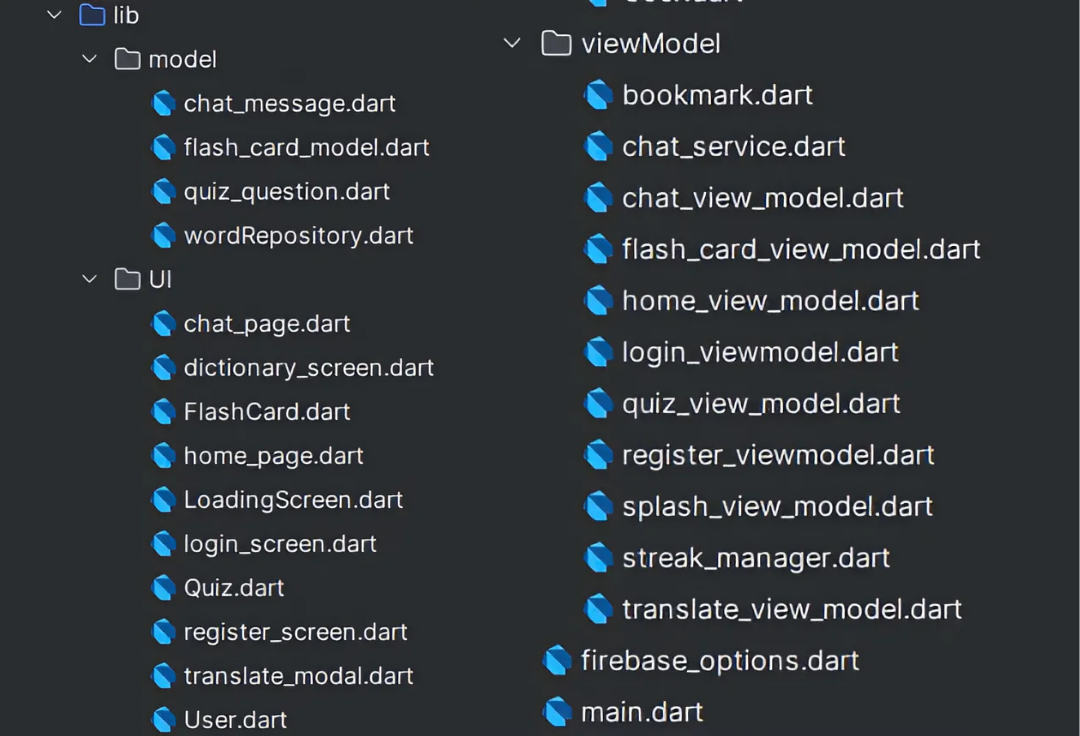
\includegraphics[width=12cm]{ảnh/16.png}
\end{center}


    \item \textbf{ Một số công nghệ và thư viện hỗ trợ quan trọng:}
    \begin{itemize}
    \item \textbf{Cloud Firestore: }Lưu trữ và đồng bộ dữ liệu người dùng (bookmark,streaks...).
    \item \textbf{SharedPreferences: }Lưu trữ dữ liệu tạm thời như lịch sử trò chuyện, trạng thái bài học.
    \item \textbf{Provider: }Quản lý trạng thái ứng dụng.
    \item \textbf{Lottie:}  Tạo hiệu ứng hoạt họa tương tác.
    \item \textbf{Google Translator API: }Hỗ trợ chức năng dịch từ/văn bản.
    \item \textbf{http, json_serializable: }Xử lý dữ liệu từ API.


    \end{itemize}
    \end{enumerate}
    

    \subsection{Kỹ thuật thiết kế giao diện người dùng (UI/UX):} 
    \begin{enumerate}
    
    \item \textbf{Thiết kế giao diện theo hướng tối giản – dễ dùng:} Ưu tiên trải nghiệm người dùng: bố cục rõ ràng, màu sắc dễ nhìn, thao tác đơn giản để người học dễ dàng tương tác mà không bị rối.
    \item \textbf{Responsive Design:} Đảm bảo giao diện hiển thị tốt trên các loại màn hình điện thoại khác nhau.
    \end{enumerate}
    
    \subsection{Phương pháp đánh giá và kiểm thử:} 
    \begin{enumerate}

    \item \textbf{Kiểm thử chức năng (Functional Testing):} Đảm bảo các chức năng chính như tra từ, tạo flashcard, trả lời câu hỏi quiz, dịch tiếng anh, chatbox AI, lưu dữ liệu người dùng hoạt động ổn định.
    \item \textbf{Kiểm thử giao diện (UI Testing):} Đánh giá khả năng tương tác, bố cục hiển thị, sự thân thiện với người dùng.
    \item \textbf{Lấy phản hồi người dùng thử nghiệm:} Cho một nhóm nhỏ sinh viên và người học thử dùng app để ghi nhận đánh giá, từ đó điều chỉnh và cải thiện sản phẩm.

\end{enumerate}
\section{ Tài liệu tham khảo}
\begin{itemize}
    \item \textbf{ }Giáo trình Phát triển ứng dụng di động với Flutter. NXB Đại học Quốc gia TP.HCM.
    \item \textbf{ }Google Developers. (2024). Flutter Documentation.
    \item \textbf{ }Firebase. (2024). Firebase Documentation.
   \item \textbf{ }UX Planet. (2023). Principles of Good UI/UX Design.
   \item \textbf{ }Google Translate API. (2024). Translation API Documentation. 
    \item \textbf{ }Reso Coder (2022). Flutter & Firebase Tutorial Series.
    \item \textbf{ }Phân tích và thiết kế phần mềm theo mô hình Agile/Scrum. Tạp chí Công nghệ Thông tin và Truyền thông, Số 15, tr. 45–52.
     \item \textbf{ }Oxford dictionary api
      \item \textbf{ }Cảm ơn Chat GPT

    \end{itemize}


\setcounter{section}{0}
\newpage
\input{slide2}
